\section{Why Deep Networks Are Hard to Train}

The previous sections established two major facts about neural networks.

\begin{itemize}
    \item They are highly expressive function classes.
    \item Their gradients can be computed efficiently by backpropagation.
\end{itemize}

These facts are essential, but they are not enough to guarantee successful learning.
A model may be expressive enough to represent a useful solution, and one may even know how to compute gradients exactly, yet optimization may still fail in practice.

\medskip

Historically, this was one of the central obstacles in deep learning.
Early neural networks were often difficult to optimize reliably, especially as depth increased.
The problem was not merely lack of computational power.
It was also the mathematical instability of training deep compositional models.

\medskip

This section explains why.
Its purpose is to create a genuine sense of difficulty.
Depth is not free.
The same layered composition that gives deep networks their expressive power also creates fragile optimization dynamics:
signals may shrink,
signals may explode,
curvature may become badly imbalanced,
and naïve gradient-based training may fail even when the desired function lies well inside the model class.

\medskip

Thus one must distinguish carefully between three statements:

\begin{itemize}
    \item the model class is expressive enough,
    \item gradients can be computed,
    \item training will succeed.
\end{itemize}

These are not equivalent.
This section is about the gap between the second and third.

\subsection*{Why depth creates difficulty}

A deep network is a repeated composition of transformations:
\[
h^{(0)}=x,
\qquad
h^{(1)}=\sigma(W^{(1)}h^{(0)}+b^{(1)}),
\qquad
\dots,
\qquad
h^{(L)}=f_\theta(x).
\]
During learning, information must flow in two directions:

\begin{itemize}
    \item \textbf{forward:} activations and representations must propagate from input to output;
    \item \textbf{backward:} gradient signals must propagate from loss to early layers.
\end{itemize}

\medskip

In a shallow model, these paths are short.
In a deep model, they are long and repeatedly transformed.
That repeated transformation can either preserve signal, attenuate it, or amplify it.
As depth grows, even mild distortion at each layer can accumulate into severe instability.

\medskip

This is the central intuition of the section:

\begin{quote}
Deeper composition increases expressive structure, but it also increases the difficulty of maintaining stable information flow.
\end{quote}

\subsection*{Nonconvexity}

One source of difficulty is the geometry of the optimization problem itself.
For a deep network, the empirical risk
\[
\widehat{R}_n(\theta)
=
\frac{1}{n}\sum_{i=1}^n \ell(f_\theta(x_i),y_i)
\]
is typically a highly nonconvex function of the parameters \(\theta\).

\medskip

This is very different from many classical models such as linear regression or logistic regression, where the objective is often convex.
In convex optimization, every local minimum is global, and the geometry is comparatively well behaved.
In deep learning, no such simple picture is available.

\medskip

The landscape of a deep network may contain:
\begin{itemize}
    \item local minima,
    \item saddle points,
    \item flat regions or plateaus,
    \item narrow valleys,
    \item directions with very different curvature.
\end{itemize}

\medskip

This does not mean that optimization is impossible.
Indeed, deep networks are trained successfully in practice.
But it does mean that training cannot rely on the clean geometric guarantees associated with convex objectives.
The parameter space is large, coupled, and geometrically intricate.

\commonconfusion{Nonconvex does \emph{not} automatically mean impossible. A nonconvex objective can still be trainable if gradients remain informative, scales are well controlled, and the optimization geometry is manageable. Conversely, even a smooth objective can be painful to optimize if gradients vanish, explode, or point through badly conditioned directions. Nonconvexity is one source of difficulty, not the whole story.}

\subsection*{Gradient propagation through depth}

The main computational difficulty of deep learning appears most clearly in the backward pass.
The chain rule says that a derivative through a composition is a product of local derivatives.
In a deep network, that means the gradient reaching an early layer is obtained by multiplying together many Jacobians.

\begin{proposition}[Gradients through depth are products of Jacobians]
Let
\[
h^{(0)}=x,
\qquad
h^{(\ell)}=F_{\ell}(h^{(\ell-1)})
\quad \text{for } \ell=1,\dots,L,
\]
and let the loss be
\[
L(x,y;\theta)=\mathcal L(h^{(L)},y).
\]
Then for every \(\ell\in\{0,\dots,L-1\}\),
\[
\nabla_{h^{(\ell)}} L
=
J_{F_{\ell+1}}(h^{(\ell)})^{\top}
J_{F_{\ell+2}}(h^{(\ell+1)})^{\top}
\cdots
J_{F_L}(h^{(L-1)})^{\top}
\nabla_{h^{(L)}}L,
\]
where \(J_{F_k}\) denotes the Jacobian of \(F_k\).
In particular, for a standard layer
\[
F_k(h)=\sigma(W^{(k)}h+b^{(k)}),
\]
we have
\[
J_{F_k}(h)=D^{(k)}W^{(k)},
\qquad
D^{(k)}=\operatorname{diag}\!\big(\sigma'(z^{(k)})\big),
\]
so backpropagation multiplies by both weight matrices and activation-derivative factors.
\end{proposition}

\begin{proof}
By the multivariable chain rule,
\[
\nabla_{h^{(L-1)}}L
=
J_{F_L}(h^{(L-1)})^{\top}\nabla_{h^{(L)}}L.
\]
Applying the same identity one step earlier gives
\[
\nabla_{h^{(L-2)}}L
=
J_{F_{L-1}}(h^{(L-2)})^{\top}\nabla_{h^{(L-1)}}L
=
J_{F_{L-1}}(h^{(L-2)})^{\top}J_{F_L}(h^{(L-1)})^{\top}\nabla_{h^{(L)}}L.
\]
Repeating this recursion yields the stated product formula.
For the layer \(F_k(h)=\sigma(W^{(k)}h+b^{(k)})\), the affine map contributes \(W^{(k)}\) and the elementwise nonlinearity contributes the diagonal derivative matrix \(D^{(k)}\), so the local Jacobian is \(D^{(k)}W^{(k)}\).
\end{proof}

This proposition is the formal anchor for the rest of the section.
It explains why depth creates both opportunity and instability: the gradient is not controlled by one local derivative, but by a long product of them.

\subsection*{A scalar toy derivation}

The same mechanism already appears in one dimension.
Consider the scalar chain
\[
h^{(0)}=x,
\qquad
h^{(\ell)}=\phi\big(a\,h^{(\ell-1)}\big),
\qquad \ell=1,\dots,L,
\]
with scalar parameter \(a\), activation \(\phi\), and scalar loss
\[
L=\mathcal L(h^{(L)}).
\]
By repeated application of the chain rule,
\[
\frac{\partial L}{\partial h^{(0)}}
=
\frac{\partial L}{\partial h^{(L)}}
\prod_{\ell=1}^{L}
\frac{\partial h^{(\ell)}}{\partial h^{(\ell-1)}}
=
\frac{\partial L}{\partial h^{(L)}}
\prod_{\ell=1}^{L}
\Big(a\,\phi'\big(a h^{(\ell-1)}\big)\Big).
\]
If the local factor is typically of size \(\rho\), meaning roughly
\[
\big|a\,\phi'(a h^{(\ell-1)})\big|\approx \rho,
\]
then
\[
\left|\frac{\partial L}{\partial h^{(0)}}\right|
\approx
\left|\frac{\partial L}{\partial h^{(L)}}\right|\rho^L.
\]
So:
\begin{itemize}
    \item if \(\rho<1\), the gradient decays exponentially with depth;
    \item if \(\rho>1\), the gradient grows exponentially with depth;
    \item if \(\rho\approx 1\), gradient scale is at least \emph{capable} of remaining stable.
\end{itemize}

\medskip

This toy derivation is deliberately simple, but the lesson is exact in spirit.
Deep learning is hard because repeated multiplication magnifies even mild layerwise imbalance.

\subsection*{Vanishing gradients}

The \emph{vanishing gradient problem} occurs when backward-propagated gradient signals become extremely small in early layers.

\medskip

At an intuitive level, this means that the loss provides only a weak learning signal to the beginning of the network.
The later layers may still update, but the earlier layers --- which are supposed to learn foundational representations --- change very slowly.

\medskip

In terms of the Jacobian product,
vanishing gradients arise when the typical singular values or effective scalar factors along the backward path are smaller than one, so that repeated multiplication contracts:
\[
\|\nabla_{h^{(\ell)}}L\| \ll \|\nabla_{h^{(L)}}L\|
\qquad\text{for early }\ell.
\]

\medskip

This is especially problematic because early layers are often the ones that should learn the most reusable and task-important features.
If they receive almost no gradient, the whole representational hierarchy becomes difficult to organize effectively.

\medskip

A useful way to think about vanishing gradients is this:
backpropagation communicates error information backward through the network.
If that communication decays exponentially with depth, then distant layers are almost cut off from the learning signal.

\subsection*{Exploding gradients}

The opposite problem is the \emph{exploding gradient problem}.
Here the repeated products in the backward pass amplify rather than suppress the signal, so that
\[
\|\nabla_{h^{(\ell)}}L\| \gg \|\nabla_{h^{(L)}}L\|
\]
for some early layers.

\medskip

When this happens, updates become numerically unstable.
Parameter changes may become excessively large, optimization may oscillate wildly, and the loss may jump unpredictably rather than decrease smoothly.

\medskip

Exploding gradients are particularly severe in deep or recurrent models, where long chains of multiplication are unavoidable.
Even when not catastrophic, they can make training extremely sensitive to learning rates and initialization scales.

\medskip

The vanishing and exploding cases are opposite in direction, but similar in spirit:
both are failures of stable signal propagation through depth.

\subsection*{Saturation of sigmoid and tanh activations}

A particularly important source of vanishing gradients comes from \emph{saturation} of activation functions.
Consider activations such as the sigmoid
\[
\sigma(z)=\frac{1}{1+e^{-z}}
\]
or the hyperbolic tangent
\[
\tanh(z).
\]
These functions flatten out in parts of their domain.
In those regions, their derivatives are small:
\[
\sigma'(z)=\sigma(z)(1-\sigma(z)),
\qquad
\tanh'(z)=1-\tanh^2(z).
\]

\medskip

Since backpropagation multiplies by these derivatives, activations that spend much time in saturated regimes strongly attenuate gradient flow.
Even if the weight matrices themselves are well behaved, repeated multiplication by near-zero activation derivatives can make gradients vanish rapidly.

\medskip

This is why the geometry of the activation function matters.
The issue is not merely that the network is nonlinear.
The issue is how the nonlinearity behaves in the regimes actually visited during training.

\begin{figure}[tbp]
\centering
\begin{minipage}[t]{0.48\textwidth}
\centering
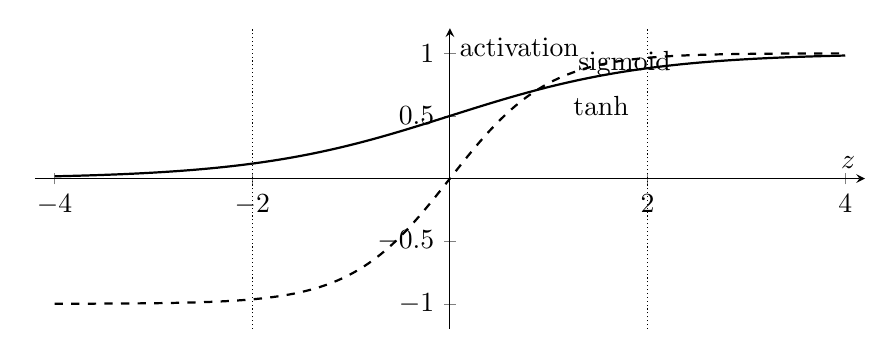
\begin{tikzpicture}
\begin{axis}[
    width=\textwidth,
    height=5.4cm,
    axis lines=middle,
    xmin=-4.2,xmax=4.2,
    ymin=-1.2,ymax=1.2,
    xlabel={$z$},
    ylabel={activation},
    xtick={-4,-2,0,2,4},
    ytick={-1,-0.5,0,0.5,1},
    domain=-4:4,
    samples=200,
    clip=false,
]
\addplot[thick] {1/(1+exp(-x))};
\addplot[thick,dashed] {tanh(x)};
\node[anchor=west] at (axis cs:1.2,0.92) {sigmoid};
\node[anchor=west] at (axis cs:1.15,0.58) {tanh};
\draw[densely dotted] (axis cs:-2,-1.2) -- (axis cs:-2,1.2);
\draw[densely dotted] (axis cs:2,-1.2) -- (axis cs:2,1.2);
\end{axis}
\end{tikzpicture}
\subcaption{Sigmoid and tanh flatten in their tails.}
\end{minipage}
\hfill
\begin{minipage}[t]{0.48\textwidth}
\centering
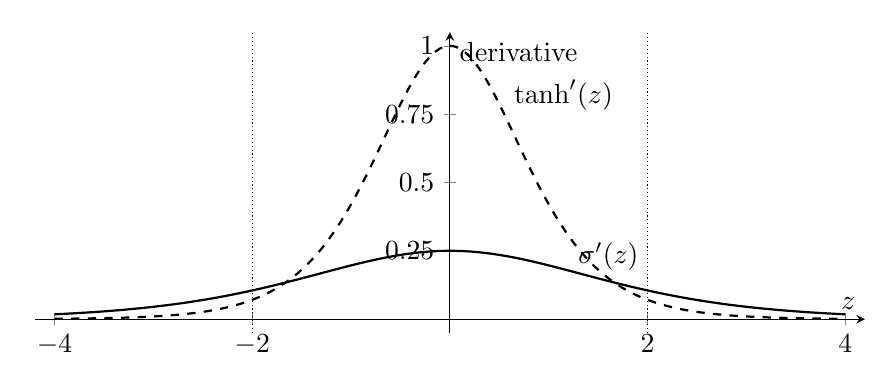
\begin{tikzpicture}
\begin{axis}[
    width=\textwidth,
    height=5.4cm,
    axis lines=middle,
    xmin=-4.2,xmax=4.2,
    ymin=-0.05,ymax=1.05,
    xlabel={$z$},
    ylabel={derivative},
    xtick={-4,-2,0,2,4},
    ytick={0,0.25,0.5,0.75,1},
    domain=-4:4,
    samples=200,
    clip=false,
]
\addplot[thick] {(1/(1+exp(-x)))*(1-1/(1+exp(-x)))};
\addplot[thick,dashed] {1-(tanh(x))^2};
\node[anchor=west] at (axis cs:1.2,0.23) {$\sigma'(z)$};
\node[anchor=west] at (axis cs:0.55,0.82) {$\tanh'(z)$};
\draw[densely dotted] (axis cs:-2,-0.05) -- (axis cs:-2,1.05);
\draw[densely dotted] (axis cs:2,-0.05) -- (axis cs:2,1.05);
\end{axis}
\end{tikzpicture}
\subcaption{Derivatives are small in the saturated regions.}
\end{minipage}
\caption{Saturation harms gradient flow. When pre-activations spend much time in the tails of sigmoid or tanh, the local derivative is small, so the backward signal is repeatedly attenuated.}
\end{figure}

Saturation also has a forward-pass interpretation.
If many units are in flat regions of the activation, then their outputs become relatively insensitive to changes in input.
The network then loses expressive responsiveness locally, while the backward signal simultaneously weakens.

\medskip

Thus saturation harms both representation dynamics and optimization dynamics.

\subsection*{Ill-conditioned optimization}

Even when gradients do not vanish or explode outright, optimization can still be very slow if the objective is badly conditioned.

\medskip

Conditioning concerns how differently the objective behaves in different parameter directions.
If one direction has very high curvature while another has very low curvature, then a single learning rate is hard to choose well:
\begin{itemize}
    \item too large a step may overshoot in steep directions,
    \item too small a step may barely move in flat directions.
\end{itemize}

\medskip

This leads to zig-zagging, oscillation, or painfully slow progress.
A familiar geometric picture is that of a narrow curved valley:
gradient descent keeps bouncing across the steep walls while making only limited progress along the shallow direction.

\begin{figure}[tbp]
\centering
\begin{minipage}[t]{0.48\textwidth}
\centering
\begin{tikzpicture}[scale=0.95]
\draw[->] (-2.4,0) -- (2.4,0) node[right] {$\theta_1$};
\draw[->] (0,-2.2) -- (0,2.2) node[above] {$\theta_2$};
\draw (0,0) ellipse (0.55 and 0.55);
\draw (0,0) ellipse (1.0 and 1.0);
\draw (0,0) ellipse (1.45 and 1.45);
\draw (0,0) ellipse (1.9 and 1.9);
\draw[thick,-{Latex[length=2mm]}] (1.6,1.55) -- (1.2,1.1);
\draw[thick,-{Latex[length=2mm]}] (1.2,1.1) -- (0.8,0.75);
\draw[thick,-{Latex[length=2mm]}] (0.8,0.75) -- (0.48,0.45);
\draw[thick,-{Latex[length=2mm]}] (0.48,0.45) -- (0.22,0.2);
\fill (1.6,1.55) circle (1.2pt);
\fill (1.2,1.1) circle (1.2pt);
\fill (0.8,0.75) circle (1.2pt);
\fill (0.48,0.45) circle (1.2pt);
\fill (0.22,0.2) circle (1.2pt);
\node at (0,-2.55) {well conditioned};
\end{tikzpicture}
\subcaption{Nearly isotropic contours permit direct progress.}
\end{minipage}
\hfill
\begin{minipage}[t]{0.48\textwidth}
\centering
\begin{tikzpicture}[scale=0.95]
\draw[->] (-2.4,0) -- (2.4,0) node[right] {$\theta_1$};
\draw[->] (0,-2.2) -- (0,2.2) node[above] {$\theta_2$};
\draw (0,0) ellipse (1.9 and 0.35);
\draw (0,0) ellipse (1.7 and 0.55);
\draw (0,0) ellipse (1.45 and 0.8);
\draw (0,0) ellipse (1.1 and 1.05);
\draw[thick,-{Latex[length=2mm]}] (1.7,1.6) -- (0.7,0.15);
\draw[thick,-{Latex[length=2mm]}] (0.7,0.15) -- (0.2,0.75);
\draw[thick,-{Latex[length=2mm]}] (0.2,0.75) -- (-0.05,0.05);
\draw[thick,-{Latex[length=2mm]}] (-0.05,0.05) -- (0.02,0.42);
\draw[thick,-{Latex[length=2mm]}] (0.02,0.42) -- (0.0,0.02);
\fill (1.7,1.6) circle (1.2pt);
\fill (0.7,0.15) circle (1.2pt);
\fill (0.2,0.75) circle (1.2pt);
\fill (-0.05,0.05) circle (1.2pt);
\fill (0.02,0.42) circle (1.2pt);
\fill (0.0,0.02) circle (1.2pt);
\node at (0,-2.55) {ill conditioned};
\end{tikzpicture}
\subcaption{Elongated contours create zig-zagging and slow progress.}
\end{minipage}
\caption{Optimization conditioning matters even when gradients exist. In poorly conditioned regions, one step size must simultaneously handle steep and flat directions, so descent can oscillate across the valley while making little progress along it.}
\end{figure}

Deep networks often suffer from such ill-conditioning because layer parameters are strongly coupled.
Changing one layer changes the distribution of inputs seen by later layers, which in turn changes the local geometry of the loss.
Thus curvature is not only anisotropic; it is also dynamically entangled across the network.

\medskip

For students, the key lesson is this:
optimization difficulty is not just about whether gradients exist.
It is also about whether those gradients point in directions that can be used effectively by finite-step algorithms.

\subsection*{Sensitivity to initialization and scale}

Because gradients propagate through long chains of transformations, deep networks are highly sensitive to how parameters are initialized.

\medskip

If initial weights are too small, then activations may collapse toward low-variation regimes and backward signals may become weak.
If initial weights are too large, activations may blow up or saturate, and gradients may become unstable.

\medskip

So initialization is not a minor implementation detail.
It is part of the mathematical condition under which learning becomes feasible.

\medskip

This sensitivity can be understood from both forward and backward viewpoints:

\paragraph{Forward scale.}
The variance or norm of activations should not grow or shrink uncontrollably across layers.

\paragraph{Backward scale.}
The magnitude of gradients should also remain within a reasonable range as they are propagated backward.

\medskip

A good initialization attempts to balance both.
This is why initialization schemes in deep learning are designed with layer width, activation type, and depth in mind.

\medskip

The broader lesson is that the trainability of a deep model depends not only on its architecture as a function class, but also on the statistical scale at which that architecture is initialized.

\subsection*{Coupled co-adaptation of layers}

A further source of difficulty is that all layers are being learned simultaneously.
A layer is not optimizing against a fixed representation supplied by previous layers.
Instead, the representations themselves are changing during training.

\medskip

This creates a moving-target problem.
When an early layer changes, it alters the effective input distribution seen by the next layer.
That layer must then readapt.
Its adaptation in turn affects the next layer, and so on.

\medskip

Thus training a deep network is not like solving a sequence of isolated subproblems.
It is a large coupled dynamical system in which many components co-adapt at once.

\medskip

This is conceptually important because it explains why depth causes difficulty even when each individual layer, considered alone, would be easy to optimize.
The challenge is not just local complexity.
It is global interaction.

\subsection*{Why naïve training can fail}

It is now possible to state the main lesson of the section more sharply.

\medskip

A deep network may fail to train well even if:
\begin{itemize}
    \item the target function lies in the hypothesis class,
    \item the loss is differentiable,
    \item backpropagation computes exact gradients.
\end{itemize}

\medskip

Failure may still occur because:
\begin{itemize}
    \item the objective is nonconvex,
    \item gradients decay through depth,
    \item gradients blow up through depth,
    \item activations saturate,
    \item curvature is badly conditioned,
    \item initialization is poorly scaled,
    \item all layers co-adapt in unstable ways.
\end{itemize}

\medskip

This is an important act of intellectual discipline.
One should not confuse representational adequacy with trainability.
A model can be expressive enough in principle and still be difficult to optimize in practice.

\subsection*{Why this difficulty mattered historically}

This section is not merely a list of technical obstacles.
It explains why the rise of deep learning took time.

\medskip

For many years, the main barrier was not the idea of multilayer representation itself.
That idea was already present.
The barrier was that deeper models were hard to train robustly and efficiently.

\medskip

Only when the field developed practical ways to stabilize optimization --- through better activations, better initialization, better architectures, better normalization, and better optimization procedures --- did deep representation learning become consistently successful at scale.

\medskip

Thus the modern toolbox should be understood as a collection of answers to genuine mathematical and computational problems, not as arbitrary tricks.

\whattoremember{Trainability problems in deep networks are not explained by one slogan. They arise from several interacting mechanisms: signal propagation through long Jacobian products, activation saturation, sensitivity to scale and initialization, ill-conditioning of the optimization geometry, and the coupled co-adaptation of layers. Nonconvexity matters, but practical trainability depends just as much on whether forward activations and backward gradients remain informative across depth.}

\subsection*{Exercises}

\begin{exercise}
Assume a scalar deep chain satisfies
\[
\frac{\partial h^{(\ell)}}{\partial h^{(\ell-1)}}=a
\qquad\text{for every }\ell=1,\dots,L,
\]
with constant scalar \(a\).
Show that
\[
\frac{\partial L}{\partial h^{(0)}}
=
a^L\frac{\partial L}{\partial h^{(L)}}.
\]
Analyze what happens as depth grows in the three regimes \(|a|<1\), \(|a|=1\), and \(|a|>1\).
\end{exercise}

\begin{exercise}
Explain in words why saturation of sigmoid or tanh harms learning.
Your answer should discuss both the forward-pass effect on responsiveness of activations and the backward-pass effect on gradient flow.
\end{exercise}

\begin{exercise}
Compare the statements ``the optimization problem is nonconvex'' and ``the optimization problem is ill conditioned.''
Why are these not the same thing?
Give an example of how a nonconvex problem could still be trainable in practice, and why even a smooth problem can be slow when curvature is badly imbalanced.
\end{exercise}

\subsection*{Notes and references}

The purpose of this section is to separate expressivity from trainability.
A deep network may be expressive enough to represent a useful solution and differentiable enough for exact gradients to be computed, yet still be hard to optimize because gradient signals decay or explode, activations saturate, curvature is badly conditioned, or layers co-adapt in unstable ways.
The next section turns to the practical response: initialization, stochastic optimization, and signal-preserving design choices that make deep learning numerically viable.
